\documentclass[herrin-thesis.tex]{subfiles}
\begin{document}

\chapter{Measuring Double-beta Decay}
\label{ch:analysis}
This is a reanalysis of the EXO-200 Run2a data, taken between September 2011 and April 2012\todo{verify}. This data has previously been used to establish a limit on \zeronu{} of \(T_{1/2}^{0\nu} > \SI{1.5e25}{\year}\) and measure the half life of \twonu{} of \(T_{1/2}^{2\nu} = (2.23 \pm 0.017 \text{ stat} \pm 0.22 \text{ sys})\times 10^{25}\si{\year}\). This analysis attempts to make a more precise measurement of  \(T_{1/2}^{2\nu}\), and also to set a limit on the Majoron-emitting modes \(0\nu\beta\beta\chi^{0}(\chi^{0})\).

There are numerous improvements over the previous analysis:
\begin{itemize}
\item Improved efficiency through identifying induction signals (\cref{sec:data_signal_extraction})
\item Improved detector homogeneity through improvements to the electron lifetime and shielding grid corrections (\cref{sec:data_corrections})
\item A calibration that takes time variation into account (\cref{sec:data_calibration})
\item Improved simulations of backgrounds in detector materials (\cref{sec:analysis_monte_carlo})
\item Incorporating position information into the signal and background models (\cref{sec:anaylsis_quantities_of_interest})
\item An improved understanding of the fiducial volume (\cref{sec:analysis_fiducial_volume})
\end{itemize}

The treatment of the data as processed in \cref{ch:data} in order to arrive at the physical results is described below.

\section{Event Selection}
\subsection{Timing-based Vetoes}
In order to reduce backgrounds (described in \cref{sec:muon_motivation}) due to cosmic-ray muons, two cuts are applied to the data:
\begin{itemize}
\item Events that occur within the \SI{25}{\ms} following a hit in a muon veto system panel are cut.
\item Events that occur within the \SI{60}{\s} following a muon passing through the TPC (identified by the method in \cref{ch:muons}) are cut. The muon events are cut themselves, as well.
\end{itemize}
These cuts are designed to remove as many cosmogenic background events as possible while not cutting a portion of the detector live time so large that the trade-off in signal-to-background ratio is not worth it.

Events occurring near each other in time are likely to be due to a decay of some radioactive contaminant, followed by another decay of a short-lived daughter. For example, the \isotope{222}{Rn} daughter \isotope{214}{Bi} \(\beta^{-}\) decays to \isotope{214}{Po}, which then \(\alpha\) decays with a \SI{164}{\micro\s} half-life.  Any event is vetoed if it occurs within \SI{\pm1}{\s} of another event.

Finally, conditions external to the detector may make the data unusable. Data from these time periods is vetoed. The most common cause is the mine evacuation siren, which is tested periodically. It is loud enough to create a large amount electronic noise through microphonic pickup. Time periods in which the siren is going off are vetoed.

The effects of all timing-based vetoes are summarized in \cref{tab:analysis_veto_effects}.

\begin{table}[htb]
\centering
\caption[Impact of timing-based vetoes]{A breakdown of the impact of the muon vetoes, TPC event-event coincidence vetoes, and the external conditions vetoes on the detector live time. Since multiple vetoes can be in effect at the same time, the combined impact of some vetoes is not simply their sum.}
\label{tab:analysis_veto_effects}
\begin{tabular}{l l l l c c}\toprule
\multicolumn{4}{c}{}							&	Time (\si{hr})	&	\%	\\\midrule
\multicolumn{4}{l}{Vetoed Time}				&	400.2		&	12.5	\\
	&\multicolumn{3}{l}{External Conditions}		&	18.4			&	0.6	\\
	&\multicolumn{3}{l}{Physics Vetoes}			&	381.8		&	11.9	\\
	&&\multicolumn{2}{l}{Muons}				&	163.5		&	5.1	\\
	&&&TPC Muon							&	144.8		&	4.5	\\
	&&&Panel Muon						&	19.6			&	0.6	\\
	&&\multicolumn{2}{l}{Event-Event Coincidence}&	236.5		&	7.4	\\
\multicolumn{4}{l}{Live Time}					&	2796.1		&	87.5	\\\midrule
\multicolumn{4}{l}{Total}						&	3196.3		&	100.0\\\bottomrule
\end{tabular}
\end{table}

\subsection{Other Vetoes}
\subsubsection{Scintillation-to-ionization ratio}
As mentioned in \cref{sec:xe_combining_ion_and_scint}, \(\alpha\) particle interactions produce more scintillation and less ionization in the liquid xenon than \(\beta\) and \(\gamma\) interactions. Therefore, events with a large scintillation-to-ionization ratio are removed from the data used for double beta decay physics. Since \isotope{222}{Rn} is a common source of \(\alpha\) particles, these decays are later used in order to constrain backgrounds due to other isotopes in the \isotope{222}{Rn} decay chain.

\subsubsection{Scintillation Timing}
Events are vetoed if they contain more than one scintillation cluster. The typical event rate in the TPC is \about{}\SI{0.1}{\Hz}, so random coincidences are rare enough that the effects of this cut on legitimate events is minuscule compared to other sources of systematic error. This eliminates \isotope{214}{Bi}-\isotope{214}{Po} coincidences, as described above, and also eliminates events in which there could be ambiguity in associating ionization signals with multiple scintillation signals. Additionally, events are vetoed if the scintillation comes too late in the waveform form ionization to have time to drift the full TPC drift length. Since the waveforms are centered around the trigger time, this does not happen in typical data, but may happen in source calibration runs.

\subsection{Fiducial Volume}
\label{sec:analysis_fiducial_volume}
\begin{figure}[htb]
\centering
	\begin{subfigure}[b]{0.48\textwidth}
	\centering
	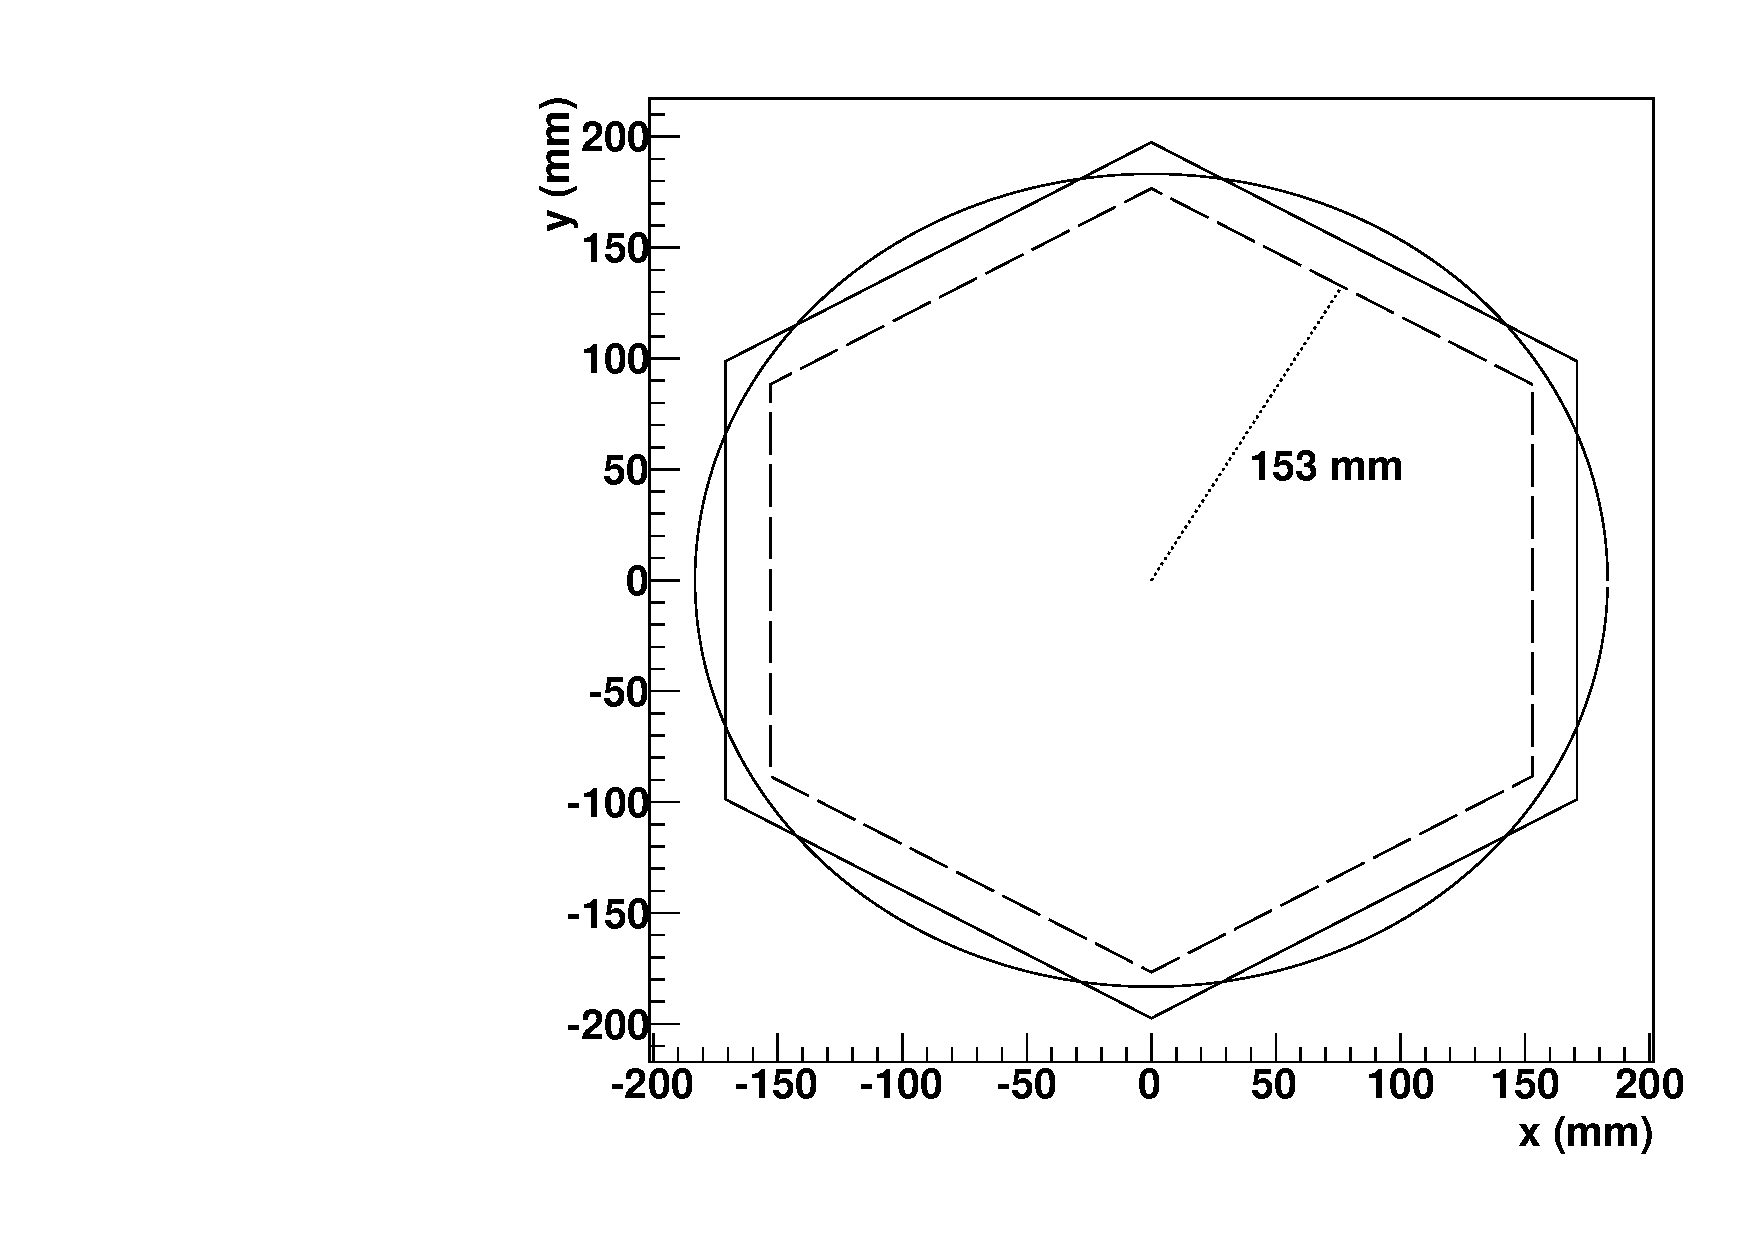
\includegraphics[width=\textwidth]{./plots/analysis_fiducial_vol_xy.pdf}
\end{subfigure}\hfill%
\begin{subfigure}[b]{0.48\textwidth}
	\centering
	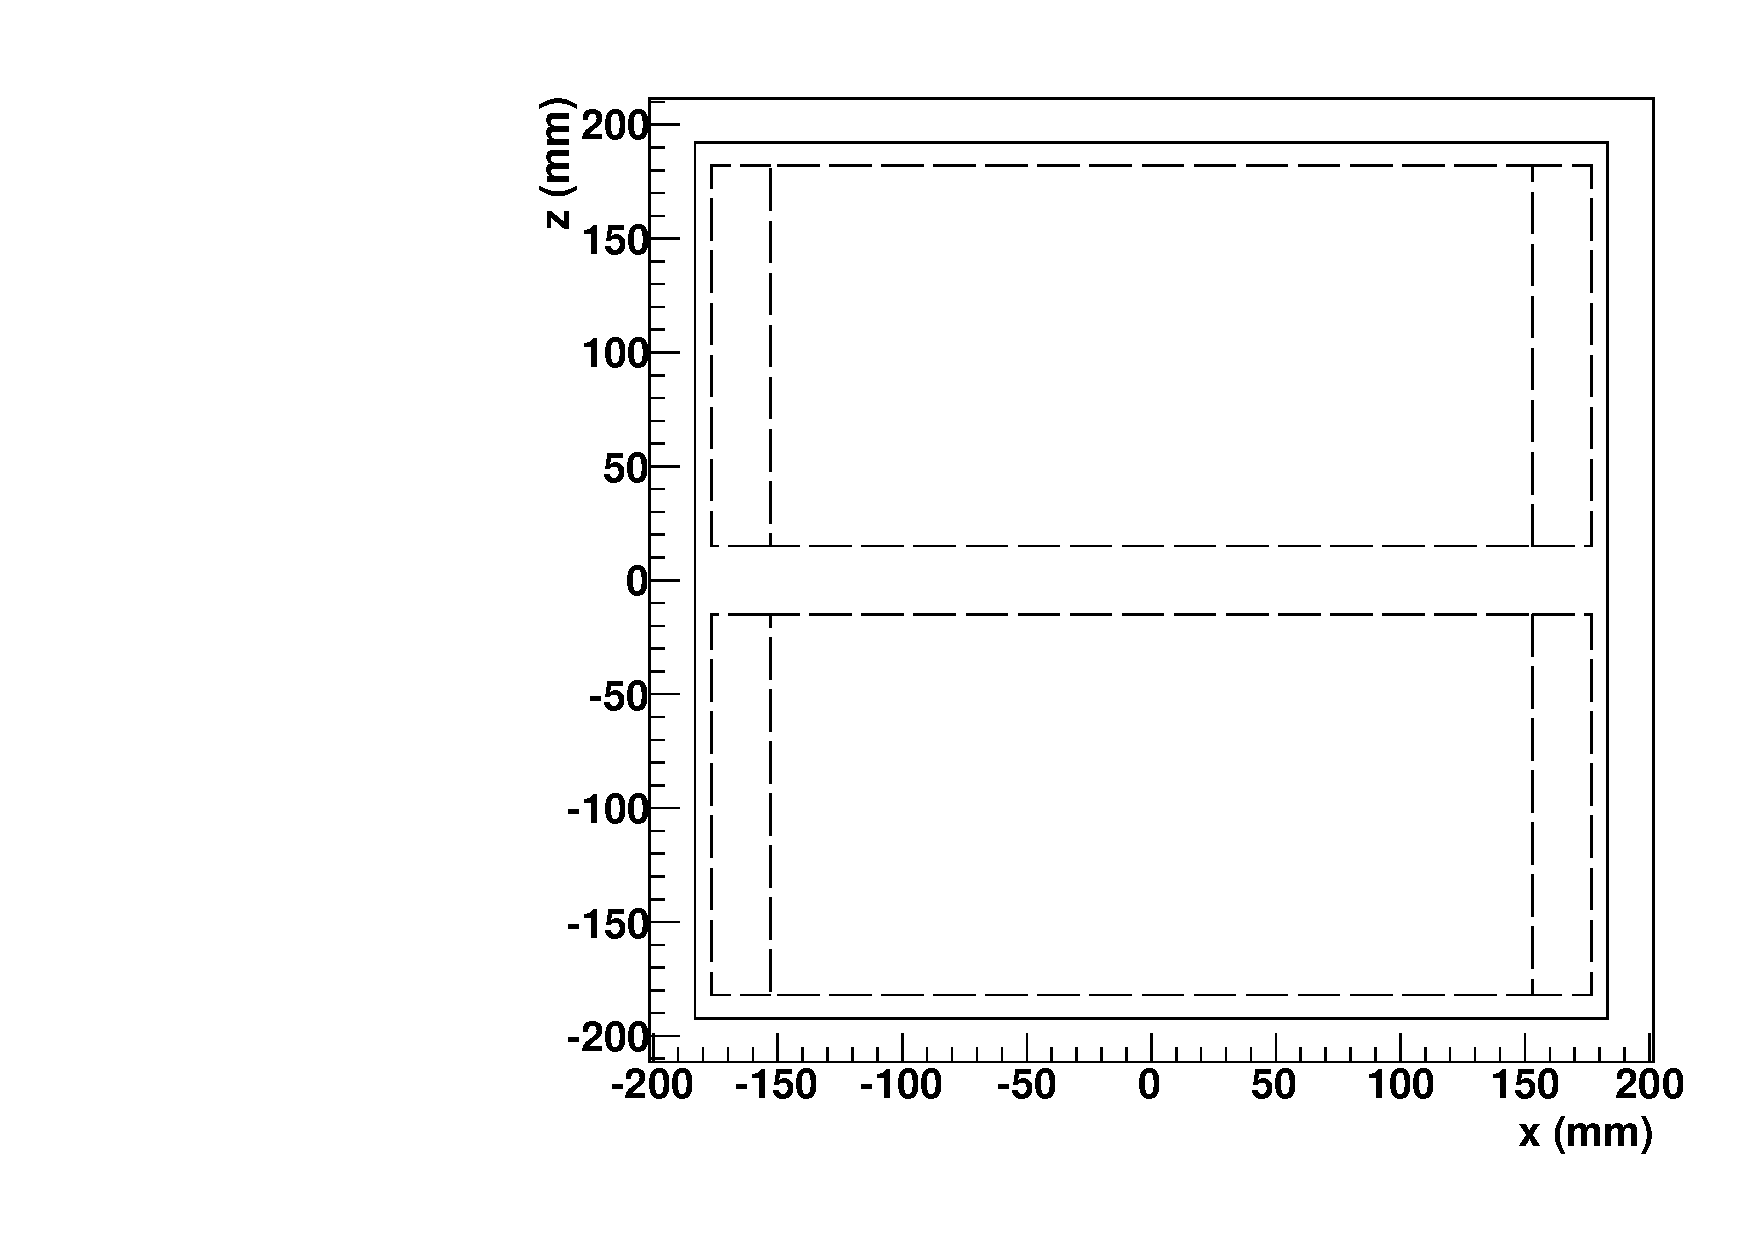
\includegraphics[width=1\textwidth]{./plots/analysis_fiducial_vol_xz.pdf}
	\end{subfigure}
\caption[Fiducial Volume]{Projections of the hexagonal fiducial volume. The dashed lines represent the fiducial volume. The solid lines are the anode wire plane and the teflon reflector. For the \(xz\) projection on the right, the two sets of vertical dashed lines are the maximum and minimum radial boundaries of the fiducial volume.}
\label{fig:analysis_fiducial_volume}
\end{figure}

All the liquid xenon within the teflon reflectors and between the anodes is ``active''. That is, ionization and scintillation in the active region are collected. However, only events within a fiducial volume are used in the analysis. This fiducial volume is a right hexagonal prism. The hexagon is coaxial with the detector and has apothem \SI{153}{\mm}. In each TPC, it begins \SI{5}{\mm} away from the cathode and extends to \SI{182}{\mm} (which is \SI{10.2}{\mm} from the \(v\) wire plane). \Cref{fig:analysis_fiducial_volume} provides an illustration. The total volume is \SI{27.1}{\litre}, which contains \SI{81.9}{\kg} of liquid xenon.

\begin{figure}[htb]
\centering
	\begin{subfigure}[b]{0.48\textwidth}
	\centering
	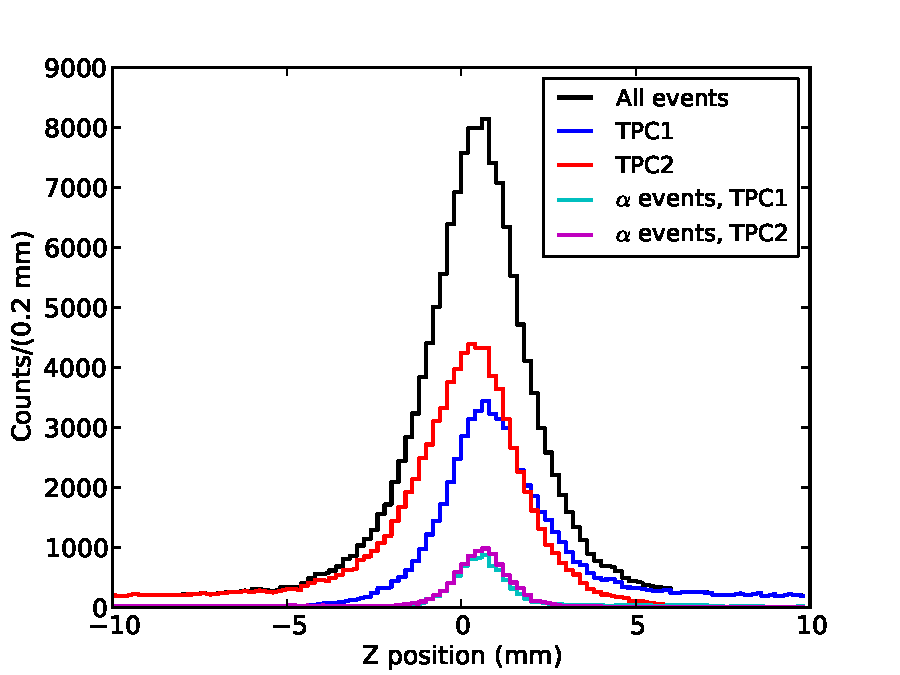
\includegraphics[width=\textwidth]{./plots/analysis_fiducial_vol_bg_cathode.pdf}
\end{subfigure}\hfill%
\begin{subfigure}[b]{0.48\textwidth}
	\centering
	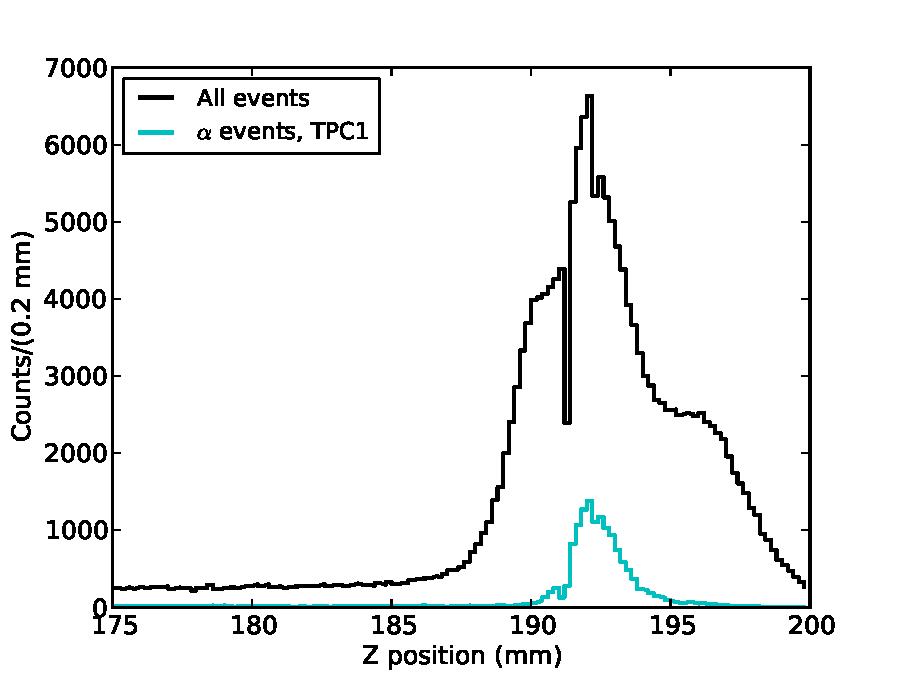
\includegraphics[width=1\textwidth]{./plots/analysis_fiducial_vol_bg_anode.pdf}
	\end{subfigure}
\caption[Increased event rates near cathode and anodes]{The choice of fiducial volume is partially motivated by the increased event rate seen near the cathode (at \(z = \SI{0}{\mm}\)) (shown left) and near the anodes (shown right; the \(v\) plane is at \(|z|=\SI{192}{\mm}\) and the \(u\) plane is at \(|z|=\SI{198}{\mm}\)). An increase is seen for both the total event rate, and for the rate of \(\alpha\) particle interactions, which suggests the increased rate is due to backgrounds. Requiring \(\SI{5}{\mm} < |z| < \SI{182}{\mm}\) puts the fiducial volume well away from the volumes that show an increased rate.}
\label{fig:analysis_fiducial_vol_bg_rates}
\end{figure}

This particular choice of fiducial volume has two chief motivations. The first is to reduce radioactive backgrounds from the detector materials. \Cref{fig:analysis_fiducial_vol_bg_rates} shows event rates near the cathode and anodes. There is nothing special about the xenon near these planes, and so the increased event rate must be due to backgrounds. The \(z\) cuts above eliminate the volumes that show higher-than-typical event rates.

\begin{figure}[htb]
\centering
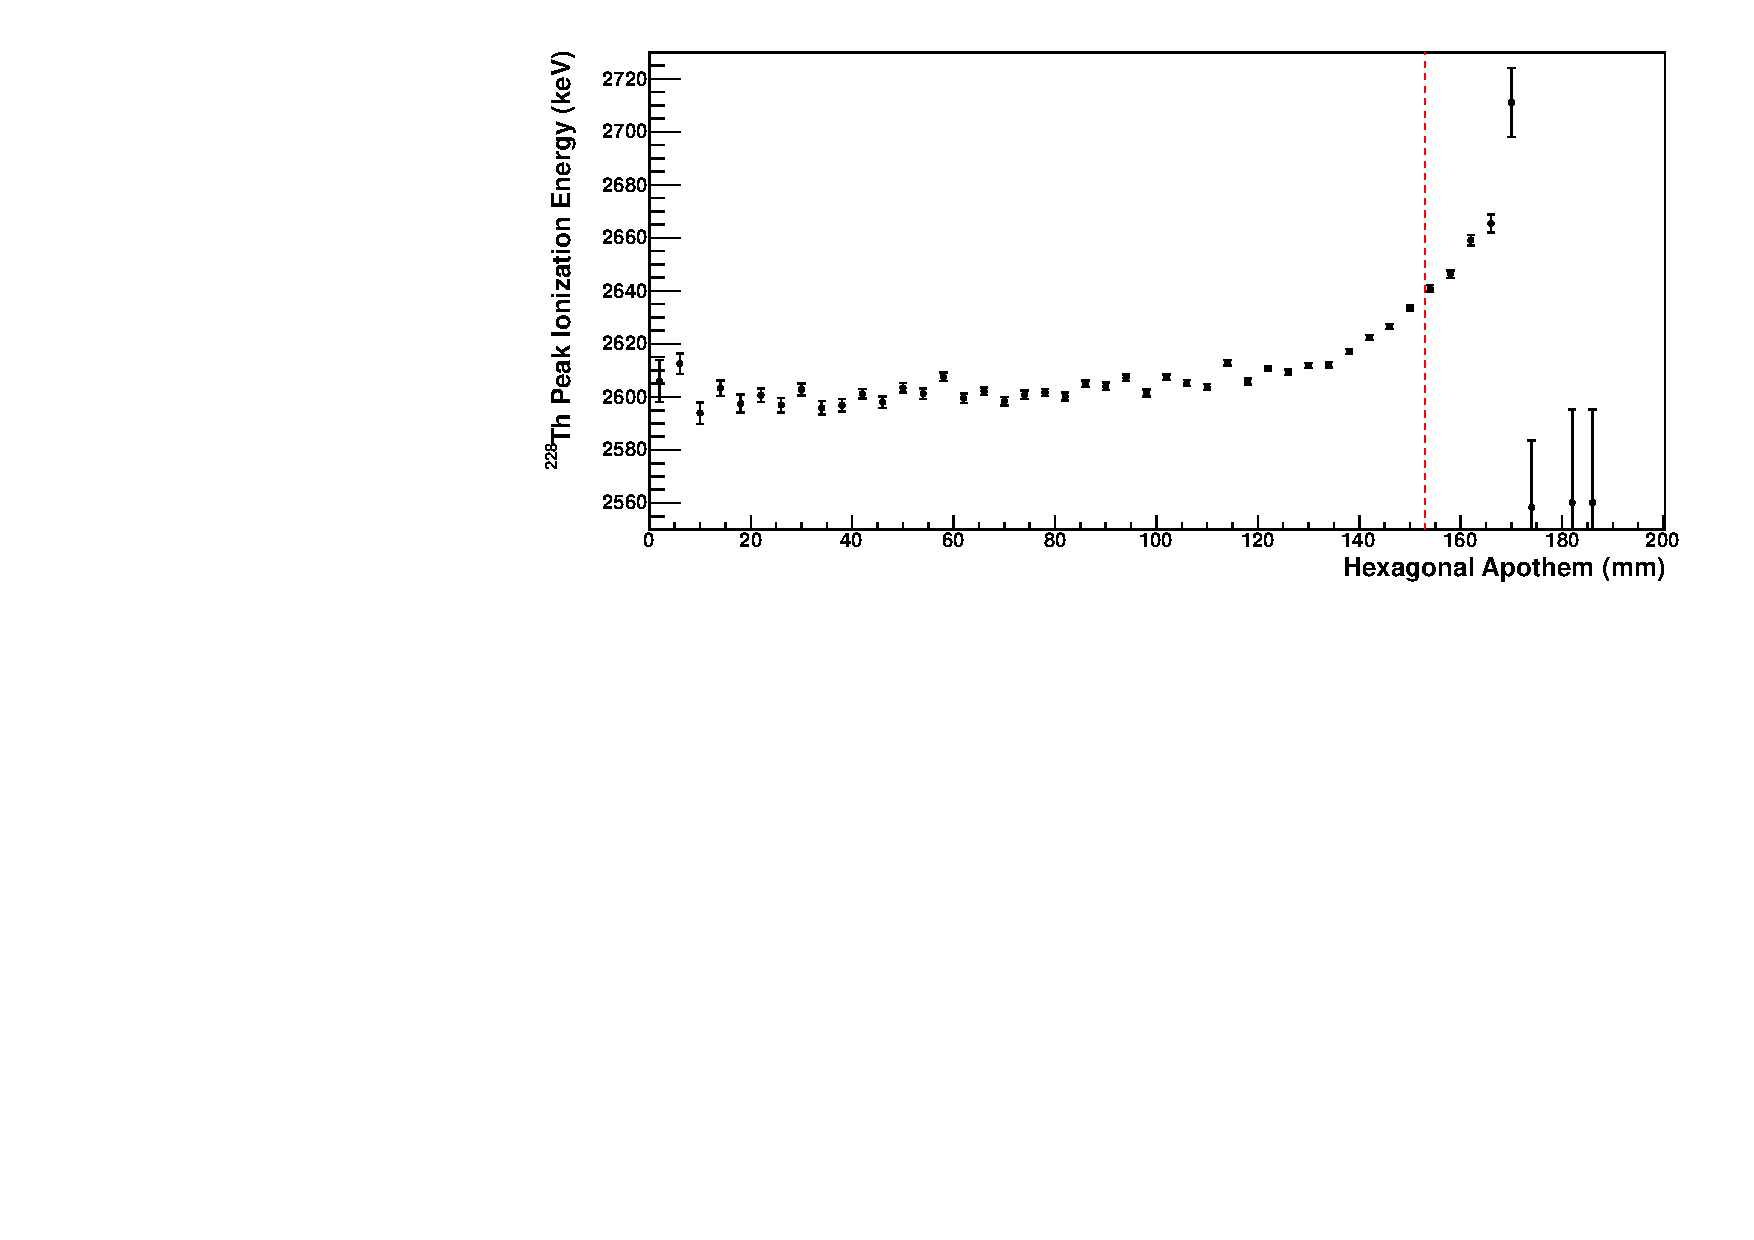
\includegraphics[width=0.8\textwidth]{./plots/analysis_fiducial_vol_transverse.pdf}
\caption[Energy response due to increasing fiducial volume apothem]{The reconstructed energy of the \SI{2615}{\keV} peak from a \isotope{228}{Th} source calibration. This is found by fitting a Gaussian + complimentary error function model to data with an increasingly large allowed fiducial volume. A larger allowed hexagonal apothem extends the fiducial volume closer and closer to the edges of the anode wire planes. The detector response begins to deviate significantly when the cut is extended above \SI{153}{\mm}, and so this is used to define the fiducial volume.}
\label{fig:analysis_fiducial_vol_bg_rates}
\end{figure}

The second motivation is to ensure a homogeneous detector response inside the fiducial volume. As shown in the previous discussion of the shielding grid correction in \cref{sec:data_grid_correction}, the correction becomes significant near \(|z|=\SI{182}{\mm}\) (see \cref{fig:data_grid_correction_fits}). Even with the correction applied, the detector response begins to diverge near that position (see \cref{fig:data_grid_correction_applied}), and so it is used as the boundary of the fiducial region. In the transverse dimension, a hexagonal cross-section is used. This matches the anode wire geometry, and so makes applying the fiducial volume cut straightforward. \Cref{fig:analysis_fiducial_vol_transverse} shows that requiring the apothem of this hexagon to be less than \SI{153}{\mm} ensures uniform energy response.

\subsection{Quantities of Interest}
\label{sec:analysis_quantities_of_interest}
Once an event passes the data quality cuts, the following quantities are calculated:
\begin{enumerate}
\item The multiplicity (single site or multiple site), using the criteria described in \cref{sec:data_topology}.
\item The event energy using the calibration obtained as described in \cref{sec:data_calibration}.
\item The ``standoff distance''. The radial distance of the cluster to the teflon reflector is calculated. So is the \(z\) distance to the \(v\) wire plane. The standoff distance is the minimum of these two distances.
\end{enumerate}

The singles site and multiple site information helps separate \(\gamma\) interactions from \(\beta\) interactions. The standoff distance describes the spatial distribution of events. For example, the distribution of \twonu{} events, since they are uniformly distributed in the detector, have a standoff distance distribution that extends to higher values. The distribution of background events from detector materials, on the other hand, peaks at small standoff distances. And, of course, the energy spectra of different types of decay are different.

\section{Monte Carlo Simulations of Signals and Backgrounds}
\label{sec:analysis_monte_carlo}

\subsection{Simulations}
The GEANT4 simulation toolkit\cite{Agostinelli:2003fk} is used in order to determine both the energy spectra and spatial distributions of various double beta decay signals and radioactive backgrounds in EXO-200. The following are simulated using a detailed model of the detector and its surroundings (see \cref{fig:analysis_geant4_detector}):
\begin{itemize}
\item Double beta decay of \xenon{136}:
	\twonu{},
	\zeronu{},
	and \(0\nu\beta\beta\chi^{0}(\chi^{0})\) for spectral indices 1, 2, 3, and 7
\item Potential backgrounds in the liquid xenon:
	\xenon{135},
	%\item \xenon{137},
	and \isotope{222}{Rn}
\item Potential backgrounds in the detector copper:
	\isotope{40}{K}, 
	\isotope{54}{Mn},
	\isotope{60}{Co},
	\isotope{65}{Zn},
	\isotope{238}{U},
	and \isotope{232}{Th}
\item \isotope{222}{Rn} in the air gap between the cryostat and lead wall
\end{itemize}

For double beta decay and background in the liquid xenon, the events are simulated uniformly in the volume of active xenon. All double beta decay modes are simulated using the Fermi function by Schenter and Vogel\cite{Schenter:1983uq}. For \isotope{222}{Rn}, there are additional complications, however. Decays of radon and daughters in the inactive xenon can emit \(\gamma\) rays that also deposit energy in the active volume. Therefore, these are simulated as well. Additionally, charged radon daughters can drift to the cathode. \isotope{214}{Bi} emits \(\gamma\) rays when it decays. The daughter \isotope{214}{Po} has a \SI{164}{\micro\s} half-life, and so both are typically eliminated by the event-event coincidence and multiple scintillation cuts. However, on the cathode, the \(\alpha\) particle from the \isotope{214}{Po} decay may go into the cathode and not be seen. Therefore, \isotope{214}{Bi} on the cathode is simulated separately.

For backgrounds in the detector copper, the TPC vessel, all internal components, the legs, and the high-voltage feedthrough are simulated as a whole. These are all modeled in the simulation, as shown in \cref{fig:analysis_geant4_detector}. It is assumed that the impurities are uniformly distributed according to copper mass. Even if some of the contamination is surface area, the thin-walled construction of EXO-200 makes this a close approximation.

\begin{figure}[htb]
\centering
	\begin{subfigure}[c]{0.58\textwidth}
	\centering
	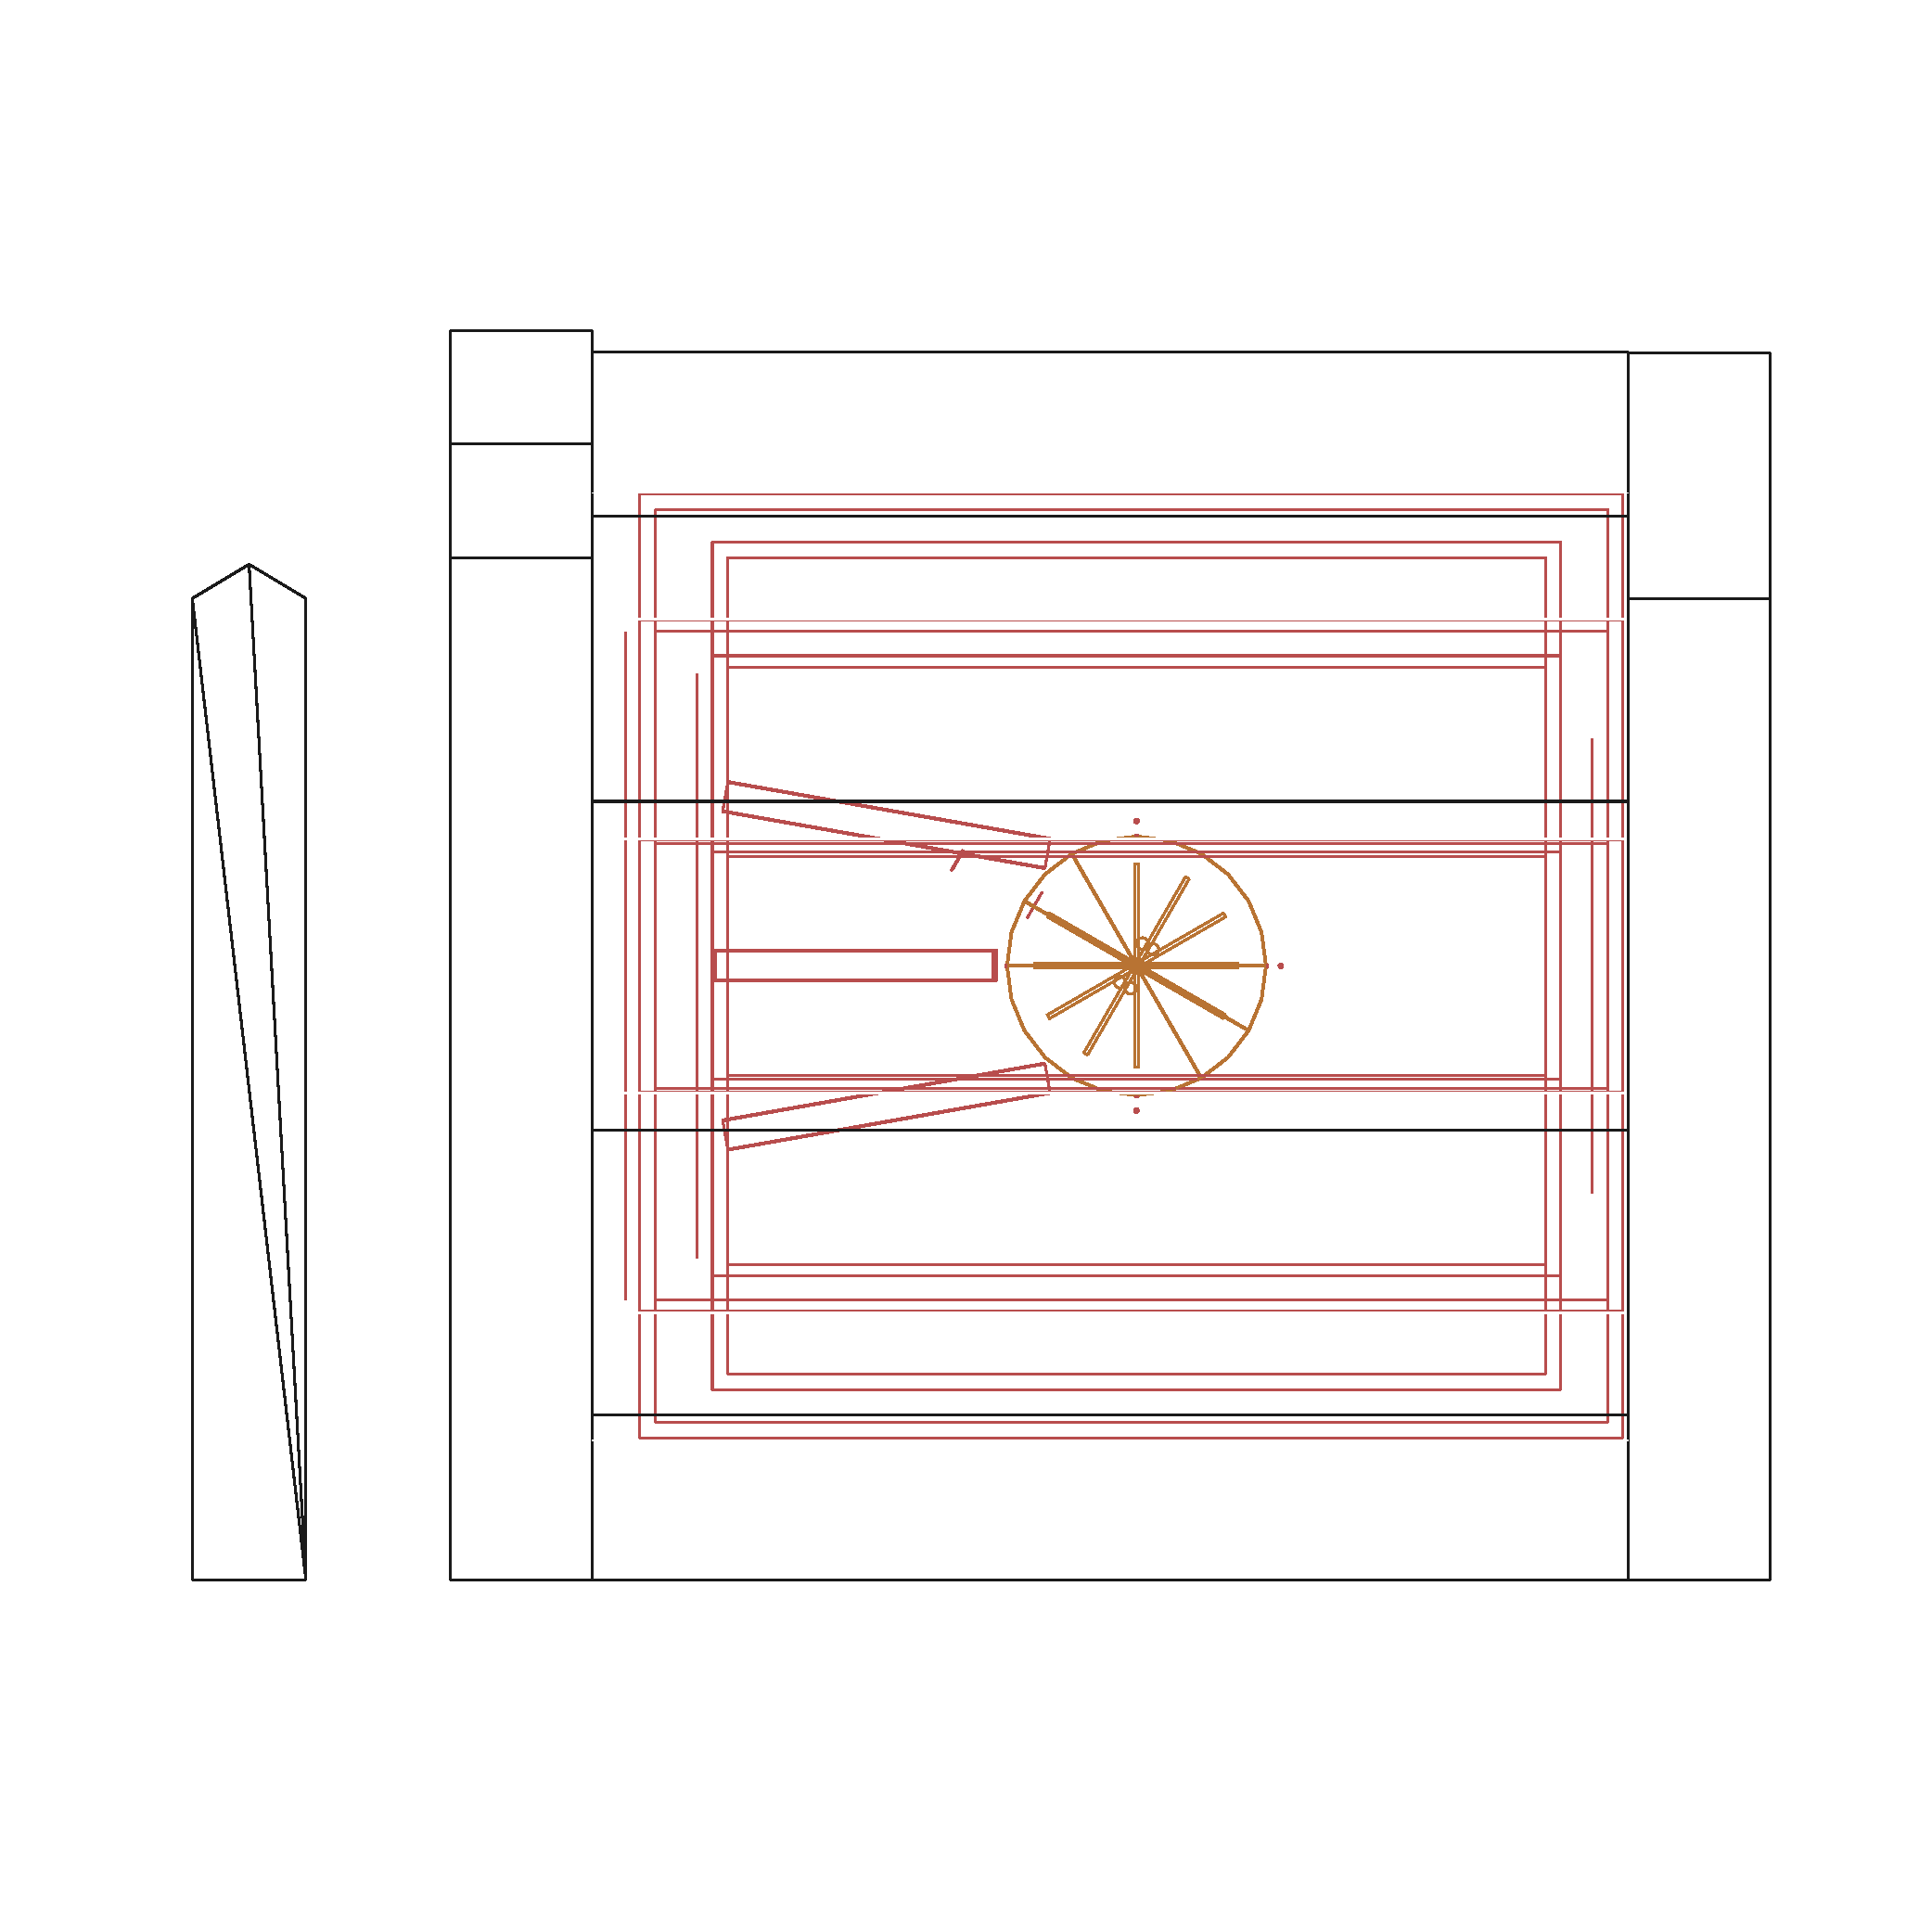
\includegraphics[width=\textwidth]{./plots/analysis_geant4_geometry_cropped.pdf}
	\end{subfigure}\hfill%
	\begin{subfigure}[c]{0.38\textwidth}
	\centering
	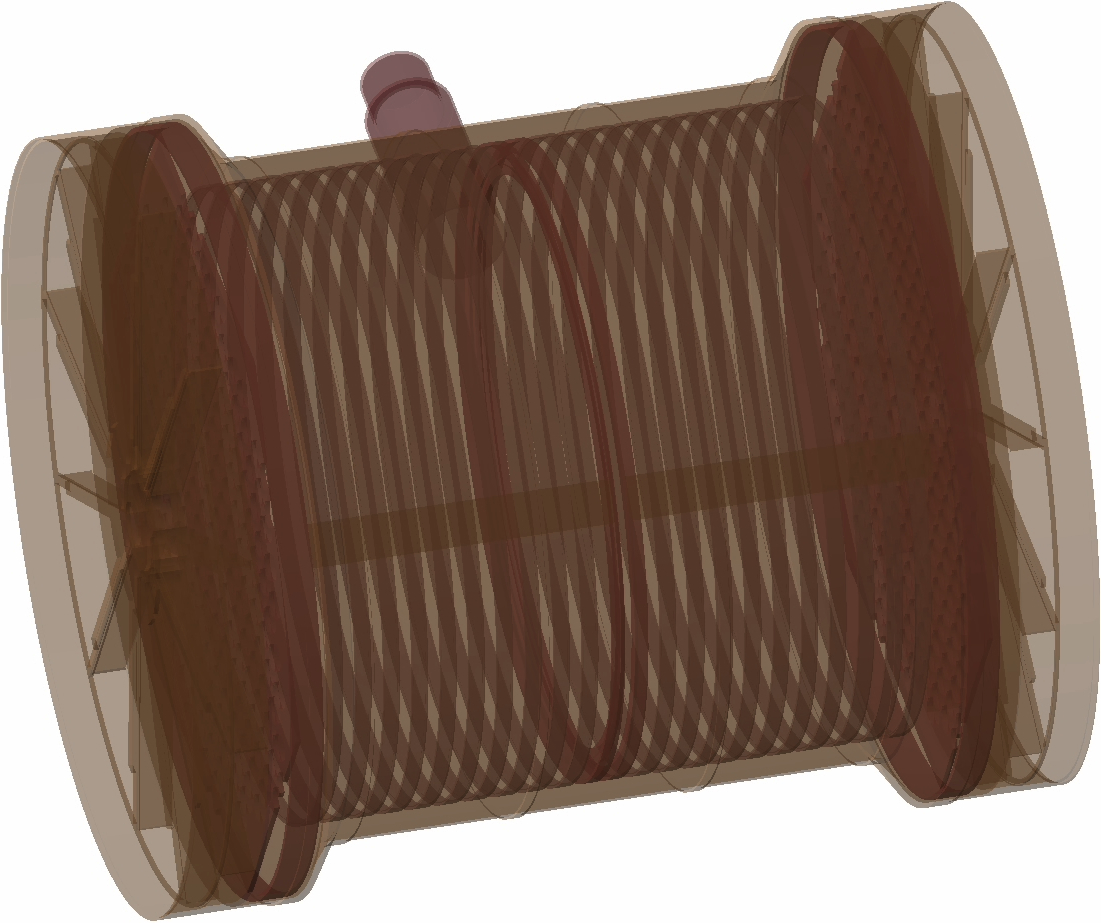
\includegraphics[width=\textwidth]{./photos/analysis_geant4_TPC_cropped.png}
	\end{subfigure}
\caption[EXO-200 geometry simulated in GEANT4]{EXO-200 as implemented in GEANT4 for simulations. The geometry incorporates the lead shielding, cryostat, HFE, and detector (shown left). The detector itself (shown right) is quite detailed in order to accurately simulate backgrounds from the detector materials.}
\label{fig:analysis_geant4_detector}
\end{figure}

In principle, backgrounds in the HFE and cryostat walls should also be simulated. However, these spectra are similar to those resulting from simulations in the detector copper. With the number of events observed by EXO-200 in the Run2a data, there is not enough statistical power to distinguish backgrounds in the detector copper from backgrounds in other, nearby materials.

Few external backgrounds (chiefly due to \isotope{40}{K}, \isotope{232}{Th}, and \isotope{238}{U} in the mine's salt walls) can penetrate the lead shielding and HFE. One notable exception is \isotope{222}{Rn}, which can exist in the air between the cryostat and lead walls. Some \(\gamma\) rays from the \isotope{214}{Bi} daughter can penetrate into the detector volume, and so this background is simulated.

\subsection{PDF Generation}
For a single event, the GEANT4 simulation provides a list of energy deposits in the liquid xenon, their positions, and their times. These must then be converted into simulations of the signals actually seen by the detector. This begins by estimating the amount of drifting ionization by using the \SI{15.6}{\eV} \(W\)-value (see \cref{sec:xe_ionization}) and the observation that \about{}\SI{80}{\percent} of ionization drifts instead of recombining in strong electric fields\cite{Aprile:1991fk}. \(\alpha\) particles have their ionization yield quenched by a factor of 0.055\cite{Aprile:1991uq}. This ionization is drifted to the anodes in small time steps, and the signals on the wires are determined using the Shockley-Ramo theorem using a 2D MAXWELL simulation of the electric fields in the detector.

The energy that doesn't go into drifting ionization goes into scintillation. The anticorrelation between ionization and scintillation is not modeled, and so the fraction of energy in scintillation is constant. The scintillation photons are distributed across the two planes in a parameterized way. All photoelectrons from the APDs are assumed to arrive instantaneously, since the scintillation signal arrives in \si{\ns}, compared to the \si{\micro\s} digitization time.

White noise is added to the ionization and scintillation signals to yield a similar signal-to-noise ratio as in the detector. They are then run through simulations of the shapers found in the detector electronics, and are digitized at \SI{1}{\MHz}, just like the real signals. The matched filter and multiple signal finder are applied to identify signals, and the signals are bundled and clustered. The process is identical to the one described in \cref{sec:data_reconstruction}. This simulates the efficiency and energy threshold effects that come from signal-finding and reconstruction, as well as the position resolution.

The final state is to form distributions in multiplicity, energy, and standoff distance that can be fit to the data collected by the detector. The multiplicity and standoff distance can be calculated directly from the reconstruction described above. For the energy, however, the true energy from Monte Carlo simulation is used. For each cluster found by the reconstruction process, the energy deposits that arrived on the wires associated with the cluster at the appropriate time are summed to get the cluster's true energy.

In order to simulate the detector energy resolution, the true energies are smeared by a parameterized resolution function given by
\begin{equation}
\sigma(E)/E = \sqrt{\frac{p_0^2}{E^2} + \frac{p_1^2}{E} + p_2^2}
\label{eq:analysis_energy_resolution}
\end{equation}
where \(p_0\) is a constant, noise-like smearing, \(p_1\) is a smearing due to counting statistics, and \(p_2\) is an energy-dependent smearing that can be due to drifting gains. These parameters are determined on a week-by-week basis by fitting a simulated calibration source spectrum to the data collected by the detector during calibration runs with that source.

The true energies from the signal and background Monte Carlo simulations are smeared according to the parameterization in \cref{eq:analysis_energy_resolution}. For each simulation, then two probability density functions (PDFs) are formed in energy and standoff distance: one for single site events, and one for multiple site events. For each simulation, the efficiency for a simulated event to make it into the final PDFs is recorded, as well as the fractional split between single site and multiple site events.

\section{Systematic Uncertainties}

\section{Constraints}

\section{Maximum Likelihood Method}

\section{Measurement of \twonu}

\subsection{Consistency Checks}

\section{Limits on \(0\nu\beta\beta\chi^0(\chi^0)\)}

\end{document}
